%%%%%%%%%%%%%%%%%%%%%%%%%%%%%%%%%%%%%%%%%
% Beamer Presentation
% LaTeX Template
% Version 1.0 (10/11/12)
%
% This template has been downloaded from:
% http://www.LaTeXTemplates.com
%
% License:
% CC BY-NC-SA 3.0 (http://creativecommons.org/licenses/by-nc-sa/3.0/)
%
%%%%%%%%%%%%%%%%%%%%%%%%%%%%%%%%%%%%%%%%%

%----------------------------------------------------------------------------------------
%	PACKAGES AND THEMES
%----------------------------------------------------------------------------------------

\documentclass{beamer}

\mode<presentation> {

% The Beamer class comes with a number of default slide themes
% which change the colors and layouts of slides. Below this is a list
% of all the themes, uncomment each in turn to see what they look like.

\usetheme{default}
%\usetheme{AnnArbor}
%\usetheme{Antibes}
%\usetheme{Bergen}
%\usetheme{Berkeley}
%\usetheme{Berlin}
%\usetheme{Boadilla}
%\usetheme{CambridgeUS}
%\usetheme{Copenhagen}
%\usetheme{Darmstadt}
%\usetheme{Dresden}
%\usetheme{Frankfurt}
%\usetheme{Goettingen}
%\usetheme{Hannover}
%\usetheme{Ilmenau}
%\usetheme{JuanLesPins}
%\usetheme{Luebeck}
%\usetheme{Madrid}
%\usetheme{Malmoe}
%\usetheme{Marburg}
%\usetheme{Montpellier}
%\usetheme{PaloAlto}
%\usetheme{Pittsburgh}
%\usetheme{Rochester}
%\usetheme{Singapore}
%\usetheme{Szeged}
%\usetheme{Warsaw}

% As well as themes, the Beamer class has a number of color themes
% for any slide theme. Uncomment each of these in turn to see how it
% changes the colors of your current slide theme.

%\usecolortheme{albatross}
%\usecolortheme{beaver}
%\usecolortheme{beetle}
%\usecolortheme{crane}
%\usecolortheme{dolphin}
\usecolortheme{dove} %fine
%\usecolortheme{fly}
%\usecolortheme{lily}
%\usecolortheme{orchid}
%\usecolortheme{rose}
%\usecolortheme{seagull}
%\usecolortheme{seahorse}
%\usecolortheme{whale}
%\usecolortheme{wolverine}

%\setbeamertemplate{footline} % To remove the footer line in all slides uncomment this line
\setbeamertemplate{footline}[page number] % To replace the footer line in all slides with a simple slide count uncomment this line

\setbeamertemplate{navigation symbols}{} % To remove the navigation symbols from the bottom of all slides uncomment this line
}

\usepackage{graphicx} % Allows including images
\usepackage{booktabs} % Allows the use of \toprule, \midrule and \bottomrule in tables

\usepackage{minted}
\usepackage{tcolorbox}
\tcbuselibrary{breakable,skins,minted}
\usepackage{etoolbox}
\usepackage{fancyvrb}

%\usepackage{listings}

%\lstset{
%  language=C,                % choose the language of the code
%  numbers=left,                   % where to put the line-numbers
%  stepnumber=1,                   % the step between two line-numbers.        
%  numbersep=5pt,                  % how far the line-numbers are from the code
%  backgroundcolor=\color{white},  % choose the background color. You must add \usepackage{color}
%  showspaces=false,               % show spaces adding particular underscores
%  showstringspaces=false,         % underline spaces within strings
%  showtabs=false,                 % show tabs within strings adding particular underscores
%  tabsize=2,                      % sets default tabsize to 2 spaces
%  captionpos=b,                   % sets the caption-position to bottom
%  breaklines=true,                % sets automatic line breaking
%  breakatwhitespace=true,         % sets if automatic breaks should only happen at whitespace
%  title=\lstname,                 % show the filename of files included with \lstinputlisting;
%}


\usepackage{subcaption}
%\usepackage{enumitem}

%\setlist[itemize,2]{label={$\star$}}

%----------------------------------------------------------------------------------------
%	TITLE PAGE
%----------------------------------------------------------------------------------------

\title[wflz]{wflz} % The short title appears at the bottom of every slide, the full title is only on the title page

\author{Jiri Hamberg} % Your name
\institute[Uni.Helsinki] % Your institution as it will appear on the bottom of every slide, may be shorthand to save space
{
Data Compression Seminar 2017 \\ % Your institution for the title page
%\medskip
%\textit{jiri.hamberg@cs.helsinki.fi} % Your email address
}
\date{20.3.2017} % Date, can be changed to a custom date

%\setbeamersize{sidebar width left=0pt}
\setbeamertemplate{sidebar left}{}

\begin{document}

%\begin{frame}
%\titlepage % Print the title page as the first slide
%\end{frame}

\frame[plain] {
	\titlepage
}

%\begin{frame}
%\frametitle{Overview} % Table of contents slide, comment this block out to remove it
%\tableofcontents % Throughout your presentation, if you choose to use \section{} and \subsection{} commands, these will automatically be printed on this slide as an overview of your presentation
%\end{frame}

%----------------------------------------------------------------------------------------
%	PRESENTATION SLIDES
%----------------------------------------------------------------------------------------

%------------------------------------------------
\section{Performance} 

%\begin{frame}
%\frametitle{Introduction}

%\begin{itemize}
%	\item Why should we measure TCP?
%	\setbeamertemplate{itemize items}[circle]	
%	\begin{itemize}
%		\item TCP is the backbone of the Internet
		
%		\item TCP needs to keep up with evolving Internet
		
%		\item Analytical models are hard 
%	\end{itemize}
%\end{itemize}

%\end{frame}
\frame {
	\frametitle{Overview}

	\begin{itemize}
		\item Simple open source C library - 837 lines of code
		\item 2 compression levels - "fast" and normal
		\item Operates in memory
		\item Pretty bad performance overall
	\end{itemize}
}

\frame {
	
	\frametitle{Performance - Wikipedia dump (95.37 MiB)}

	\begin{figure}
	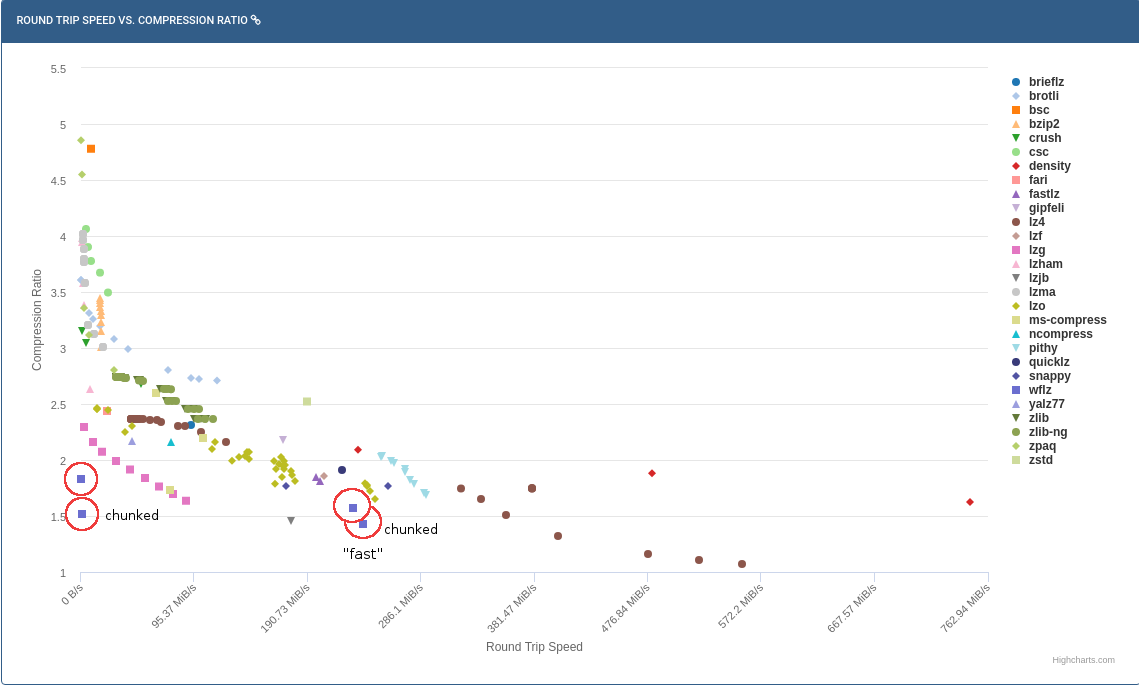
\includegraphics[width=1.0\textwidth]{img/wikipedia_edited.png}
\end{figure}
	
	
}

\frame {
	
	\frametitle{Performance - C source code (10.89 KiB)}

	\begin{figure}
	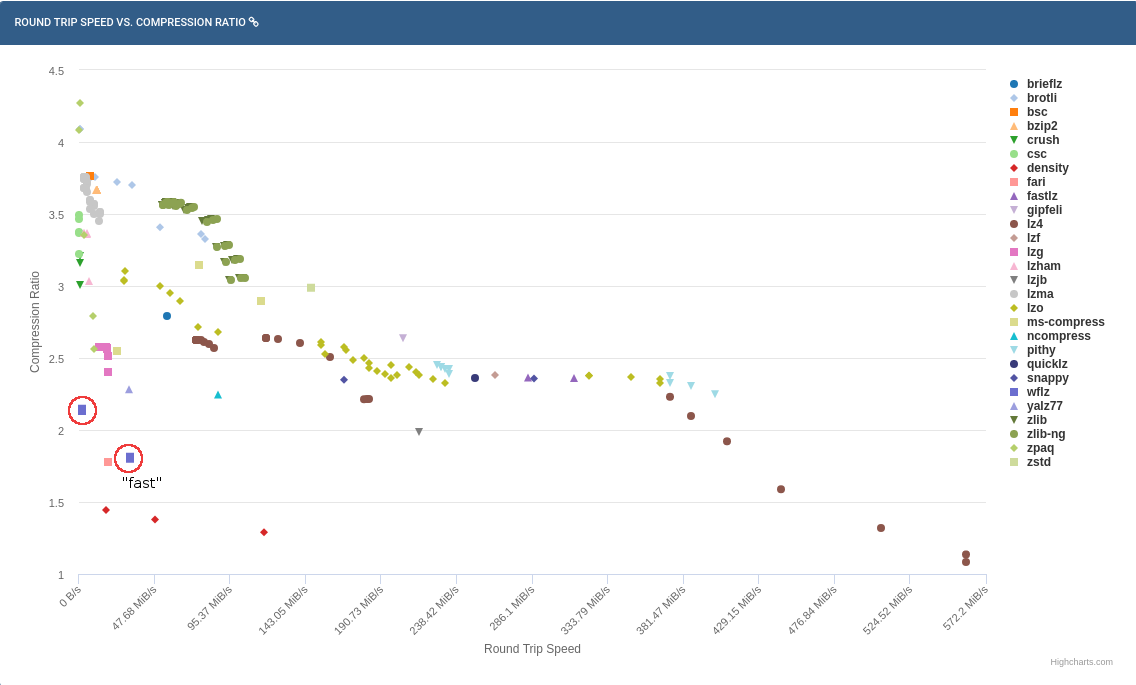
\includegraphics[width=1.0\textwidth]{img/c_edited.png}
	\end{figure}
	
}


\frame {
	
	\frametitle{Performance - xml files (5.1 MiB)}

	\begin{figure}
	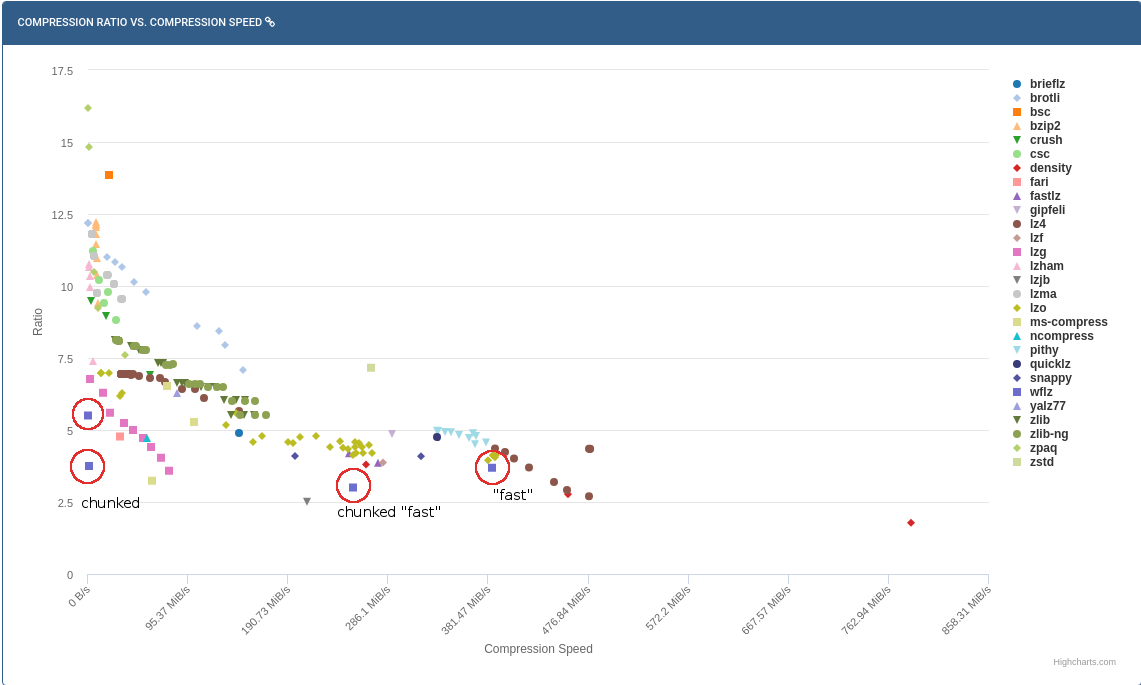
\includegraphics[width=1.0\textwidth]{img/xml_edited.png}
	\end{figure}
	
}

\section{Implementation} 

\begin{frame}
	\frametitle{Compression Format}
	
	\begin{itemize}
		\item Blocks and literals  
		\item Block consists of \textbf{distance} to reference, \textbf{length} of the reference and \textbf{number of literals} before next block
	\end{itemize}
	% typedef wfLZ_Block 
	\inputminted[firstline=49, lastline=54, breaklines]{c}{wflz/wfLZ.c}	
	
\end{frame}

\begin{frame}
	\frametitle{Compression ("fast")}
	
	\begin{enumerate}
		\item Read input one byte at a time
		\item Maintain hash table (of next four bytes at every position)
		\item Check longest match between \textit{current position} and \textit{hashtable[ hash(currentPos) ]}
		\begin{enumerate}
			\item If match is longer than than block size (4 bytes), and not too far away (distance stored in 2 bytes), write new block
			\item Otherwise write new literal
		\end{enumerate}
	\end{enumerate}
\end{frame}


\begin{frame}
	\frametitle{Compression (normal)}
	
	\begin{itemize}
		\item Like "fast" compression but instead of only checking longest match at \textit{hashtable[ hash(currentPos) ]}
		\begin{itemize}
			\item Find the best match in range \[ [\textit{currentPos} - \textit{maxMatchDist}, \textit{hashtable[ hash(currentPos) ]}] \]
		\end{itemize}
		\item Guarantees that best match is found, but is very slow
		\item For example, with dataset "dickens", wflz achieved compression speed 19.5Kib/s and ratio 1.71 whereas the fastest compressor, density achieved compression speed 227.75Mib/s (4 orders of magnitude!) and compression ratio 1.75
	\end{itemize}		 

\end{frame}

\begin{frame}
	%iterate over window to find best match
	\inputminted[fontsize=\footnotesize, tabsize=2, firstline=356, lastline=374, breaklines]{c}{wflz/wfLZ.c}	
\end{frame}


\begin{frame}
	\frametitle{Decompression}
	
	\begin{itemize}
		\item Basic LZ-decompression
		\item Uses some minor tricks to improve copy speed
		\begin{itemize}
			\item Duff's Device (loop unrolling) (I wonder if this is actually any faster than \textit{memcpy} on most platforms though)
			
		\end{itemize}		

	\end{itemize}
		
\end{frame}

\begin{frame}
	\frametitle{Duff's Device (Yes, this is valid C)}	
	
	\inputminted[fontsize=\footnotesize, tabsize=2, firstline=582, lastline=594, breaklines]{c}{wflz/wfLZ.c}	
	
\end{frame}


\begin{frame}
	\frametitle{Other tricks}
	\begin{itemize}
		\item Use of the \textit{restrict} C99-keyword for compiler optimizations 
	\end{itemize}
\end{frame}


\end{document} 
